\section*{\lr{2.7} صداپذیری و کاملیت \lr{(Soundness and Completeness)}}

    ساخت جدول معنایی یک فرایند کاملاً رسمی است. تجزیهٔ فرمول تنها مبتنی بر خواص نحوّی آن است: اپراتور اصلی فرمول و—در صورت منفی بودن—اپراتور اصلی فرمول منفی‌شده. تا کنون چند مثال برای انگیزهٔ جدول معنایی ارائه کردیم، اما صحت الگوریتم (ارتباط خروجی نحوی جدول با مفهوم معناشناختی ارزش صدق) را هنوز اثبات نکرده‌ایم. در این بخش نشان می‌دهیم که الگوریتم دقیقاً زمانی گزارش می‌دهد که فرمول ارضاپذیر یا ناتوان از ارضا است که مدل وجود دارد یا ندارد.
    
    روش‌های اثبات این بخش بسیار اهمیت دارد، زیرا در سیستم‌های منطقی دیگر بارها به‌کار گرفته می‌شوند.
    
    \begin{theorem}[قضیه \lr{2.67} صداپذیری و کاملیت]
      بگذارید $\mathscr{T}$ یک جدول تکمیل‌شده برای فرمول $A$ باشد. آنگاه:
      \[
      .\text{ ناتوان از ارضا است} A
      \;\Longleftrightarrow\;
      .\text{ بسته است} \mathscr{T}
      \]
    \end{theorem}
    
    از این قضیه چند نتیجهٔ مهم به‌دست می‌آید:
    
    \begin{corollary}[نتیجه‌گیری \lr{2.67}]
      فرمول $A$ ارضاپذیر است \emph{اگر و تنها اگر} $\mathscr{T}$ باز باشد.
    \end{corollary}
    
    \begin{proof}
      $A$ ارضاپذیر است $\iff$ (به‌تعریف) $A$ ناتوان از ارضا نیست  
      $\iff$ (با قضیهٔ \lr{2.67}) $\mathscr{T}$ بسته نیست  
      $\iff$ (به‌تعریف) $\mathscr{T}$ باز است.
    \end{proof}
    
    \begin{corollary}[نتیجه‌گیری \lr{2.68}]
      فرمول $A$ همگانی‌صادق (valid) است \emph{اگر و تنها اگر} جدول معنایی برای $\neg A$ بسته شود.
    \end{corollary}
    
    \begin{proof}
      $A$ همگانی‌صادق است  
      $\iff$ $\neg A$ ناتوان از ارضا است  
      $\iff$ جدول $\neg A$ بسته می‌شود.
    \end{proof}
    
    \begin{corollary}[نتیجه‌گیری \lr{2.70}]
      روش جدول معنایی یک رویهٔ تصمیم \lr{(decision procedure)} برای همگانی‌صدقی در منطق گزاره‌ای است.
    \end{corollary}
    
    \begin{proof}
      برای هر فرمول گزاره‌ای $A$، به کمک قضیهٔ \lr{2.66} ساخت جدول $\neg A$ پایان‌پذیر است و جدول تکمیل‌شده به‌دست می‌آید. از نتیجه‌گیری \lr{2.69} نتیجه می‌شود که  
      $A$ همگانی‌صادق $\iff$ جدول $\neg A$ بسته است.
    \end{proof}
    
    سمت مستقیم نتیجه‌گیری \lr{2.69} را \emph{کاملیت} (completeness) می‌نامند: اگر $A$ همگانی‌صادق باشد، با ساخت جدول برای $\neg A$ حتماً آن جدول بسته می‌شود.  
    جهت عکس را \emph{صداپذیری} (soundness) می‌گویند: هر فرمولی که جدول‌سازی آن را همگانی‌صادق اعلام کند (چون جدول $\neg A$ بسته است) واقعاً همگانی‌صادق است. در منطق، معمولاً اثبات صداپذیری آسان‌تر از اثبات کاملیت است؛ زیرا قواعد سیستم را طوری انتخاب می‌کنیم که آشکارا صداپذیر باشند، ولی سخت بتوانیم اطمینان یابیم که هیچ قاعدهٔ مفقودی نداریم که برای کاملیت ضروری باشد.
    
    به‌عنوان مثال، الگوریتم ضعیف زیر صداپذیر اما کاملاً ناقص است:
    
    \paragraph{الگوریتم \lr{2.71} \lr{(Incomplete decision procedure for validity)} \\}  
    \textbf{ورودی:} فرمول $A$ در منطق گزاره‌ای \\
    \textbf{خروجی:} گزارش «$A$ همگانی‌صادق نیست.»
    
    \begin{example}[مثال \lr{2.72}]
    اگر قاعدهٔ مربوط به $\neg(A_1 \lor A_2)$ را حذف کنیم، ساخت جدول هنوز صداپذیر خواهد بود، اما کاملیت را از دست می‌دهد. برای مثال فرمول واضحاً همگانی‌صادق
    \[
    A = \neg p \lor p
    \]
    را در نظر بگیرید. ریشهٔ جدول با $\neg A = \neg(\neg p \lor p)$ برچسب می‌خورد، اما هیچ قاعده‌ای برای تجزیهٔ این فرمول موجود نیست و بنابراین جدول بسته نمی‌شود، درحالی‌که $A$ به‌راستی همگانی‌صادق است.
    \end{example}

\subsection*{\lr{2.7.1} اثبات درستی}
  
  \begin{theorem}
  اگر جدول (tableau) \(\mathscr{T}\) برای فرمول \(A\) بسته شود، آنگاه \(A\) نارضایت‌پذیر \lr{unsatisfiable} است.
  \end{theorem}
  
  ما قضیه‌ای کلی‌تر را اثبات می‌کنیم:
  
  \begin{theorem}
  اگر زیر‌درخت \(\mathscr{T}_n\)، که در گرهٔ \(n\) از \(\mathscr{T}\) ریشه دارد، بسته باشد، آنگاه مجموعهٔ فرمول‌های \(U(n)\) که برچسب گرهٔ \(n\) است، نارضایت‌پذیر است.
  \end{theorem}
  
  درستیِ جدول (soundness) حالت خاصی از این قضیه است هنگامی که \(n\) همان گرهٔ ریشه باشد.
  
  برای سادگی اثبات، فرض می‌کنیم که فقط دو شکل از فرمول‌های \(\alpha\) و \(\beta\) داریم:
  \[
  \alpha\colon A_1 \land A_2,
  \qquad
  \beta\colon B_1 \lor B_2.
  \]
  
  \begin{proof}
  با استقرا بر ارتفاع \(h_n\) گرهٔ \(n\) در زیر‌درخت \(\mathscr{T}_n\).
  
  \textbf{قضیهٔ پایه} (\(h_n = 0\)).  
  اگر \(h_n=0\)، آنگاه \(n\) یک برگه (leaf) است و چون \(\mathscr{T}_n\) بسته است، در برچسب \(U(n)\) حتماً یک جفت متضاد از لیترال‌ها وجود دارد. بنابراین \(U(n)\) نارضایت‌پذیر است.
  
  \textbf{فرض استقرا}.  
  فرض کنید برای هر گرهٔ \(m\) با ارتفاع کمتر از \(h_n\) داریم:
  \[
  \forall m,\;h_m < h_n,\;\bigl[\mathscr{T}_m\ \text{بسته}\bigr]\;\Longrightarrow\;U(m)\ \text{نارضایت‌پذیر}.
  \]
  
  \textbf{گام استقرایی}.  
  حال گرهٔ \(n\) را در نظر بگیرید که \(h_n>0\). از آنجا که \(\mathscr{T}_n\) بسته است، حتماً روی \(n\) یکی از دو قاعدهٔ \(\alpha\) یا \(\beta\) اعمال شده است:
  \begin{center}
    \begin{latin}
      \resizebox{0.35\textwidth}{!}{
      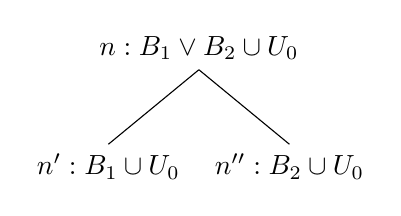
\begin{tikzpicture}[
        level distance=1.5cm,
        sibling distance=1.5cm,
        level 1/.style={sibling distance=2.3cm},
        edge from parent path={(\tikzparentnode.south) -- (\tikzchildnode.north)}
      ]
      \node {$n: {B_1 \lor B_2} \cup U_0$}
        child { 
          node {$n': {B_1} \cup U_0$}
        }
        child { 
          node {$n'': {B_2} \cup U_0$}
        };
      \end{tikzpicture}
      }  
    \hfill
    \resizebox{0.35\textwidth}{!}{
      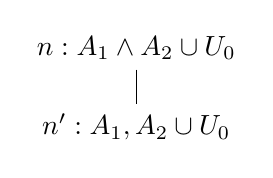
\begin{tikzpicture}[
        level distance=1cm,
        sibling distance=2.5cm,
        level 1/.style={sibling distance=2.5cm},
        level 2/.style={sibling distance=2.7cm},
        edge from parent path={(\tikzparentnode.south) -- (\tikzchildnode.north)}
      ]
      \node {$n: {A_1 \land A_2} \cup U_0$}
        child { node {$n': {A_1, A_2} \cup U_0$} };
      \end{tikzpicture}
      }
    \end{latin}
  \end{center}
  \begin{enumerate}[1)]
    \item \(\alpha\)\;  
      اگر قاعدهٔ \(\alpha\) (برای \(A_1\land A_2\)) روی \(n\) اعمال شده باشد، آنگاه
      \[
        U(n)=\{\,A_1\land A_2\}\cup U_0,
        \quad
        U(n')=\{\,A_1,\,A_2\}\cup U_0,
      \]
      و \(\mathscr{T}_{n'}\) نیز بسته است. از آنجا که ارتفاع \(n'\) برابر \(h_n-1\) است، به‌موجب فرض استقرا \(U(n')\) نارضایت‌پذیر است.  
      برای اثبات نارضایت‌پذیری \(U(n)\)، هر تفسیر دلخواه \(\mathscr{I}\) را در نظر بگیرید:
      \begin{itemize}
        \item اگر برای بعضی \(A_0\in U_0\)، \(v_{\mathscr{I}}(A_0)=F\)، چون \(U_0\subset U(n)\)، نتیجه می‌شود \(U(n)\) نارضایت‌پذیر است.
        \item در غیر این صورت \(v_{\mathscr{I}}(A_0)=T\) برای همهٔ \(A_0\in U_0\). چون \(U(n')\) نارضایت‌پذیر است، باید \(v_{\mathscr{I}}(A_1)=F\) یا \(v_{\mathscr{I}}(A_2)=F\).  
          اگر \(v_{\mathscr{I}}(A_1)=F\)، آنگاه
          \[
            v_{\mathscr{I}}(A_1\land A_2)=F,
          \]
          و چون \(A_1\land A_2\in U(n)\)، \(U(n)\) نارضایت‌پذیر است. (استدلال مشابه برای \(v_{\mathscr{I}}(A_2)=F\).)
      \end{itemize}
  
    \item \(\beta\)\;  
      اگر قاعدهٔ \(\beta\) (برای \(B_1\lor B_2\)) روی \(n\) اعمال شده باشد، آنگاه
      \[
        U(n)=\{\,B_1\lor B_2\}\cup U_0,\quad
        U(n')=\{\,B_1\}\cup U_0,\quad
        U(n'')=\{\,B_2\}\cup U_0,
      \]
      که هر دو \(\mathscr{T}_{n'}\) و \(\mathscr{T}_{n''}\) بسته‌اند و ارتفاع‌شان کمتر از \(h_n\) است. بنابراین \(U(n')\) و \(U(n'')\) نارضایت‌پذیرند.  
      برای هر تفسیر \(\mathscr{I}\):
      \begin{itemize}
        \item اگر برای بعضی \(B_0\in U_0\)، \(v_{\mathscr{I}}(B_0)=F\)، چون \(U_0\subset U(n)\)، آنگاه \(U(n)\) نارضایت‌پذیر است.
        \item وگرنه \(v_{\mathscr{I}}(B_0)=T\) برای همهٔ \(B_0\in U_0\).  
          از نارضایت‌پذیری \(U(n')\) و \(U(n'')\) داریم \(v_{\mathscr{I}}(B_1)=F\) و \(v_{\mathscr{I}}(B_2)=F\).  
          بنابراین
          \[
            v_{\mathscr{I}}(B_1\lor B_2)=F,
          \]
          و چون \(B_1\lor B_2\in U(n)\)، \(U(n)\) نارضایت‌پذیر است.
      \end{itemize}
  \end{enumerate}
  
  در هر دو حالت، نشان دادیم که اگر زیر‌درختهای فرزندان \(n\) بسته باشند، آنگاه \(U(n)\) نیز نارضایت‌پذیر است. این کامل‌کنندهٔ گام استقرایی است.
  
  بنابراین، به‌موجب اصل استقرا، برای هر گره \(n\)، اگر زیر‌درخت \(\mathscr{T}_n\) بسته باشد، آنگاه \(U(n)\) نارضایت‌پذیر است. حالت ویژه برای گرهٔ ریشه (\(n=\text{root}\)) اثبات می‌کند که اگر کل جدول \(\mathscr{T}\) بسته شود، آنگاه فرمول اولیه \(A\) نارضایت‌پذیر است.
  \end{proof}
\subsection*{\lr{2.7.2} اثبات کامل بودن \lr{(Completeness)}}
  
  \begin{theorem}
    اگر فرمول \(A\) نارضایت‌پذیر باشد، آنگاه هر جدولی (tableau) که برای \(A\) ساخته شود، بسته می‌شود.
  \end{theorem}
  
  برای اثبات، به‌جای مستقیم نشان می‌دهیم:
  
  \begin{corollary}[نتیجه گیری \lr{2.68}]
    اگر جدولی برای \(A\) باز باشد (یعنی دارای حداقل یک شاخهٔ باز)، آنگاه \(A\) برآورده‌پذیر (satisfiable) است.
  \end{corollary}
  
  روش کار در چهار گام اصلی است:
  \begin{enumerate}[1)]
    \item تعریف مجموعهٔ هینتیکا \lr{(Hintikka set)}.
    \item اثبات اینکه اجتماع برچسب‌های گره‌های یک شاخهٔ باز، یک مجموعهٔ هینتیکا است.
    \item اثبات اینکه هر مجموعهٔ هینتیکا برآورده‌پذیر است.
    \item نشان دادن اینکه خود فرمول \(A\) (برچسب ریشه) در آن مجموعه حضور دارد.
  \end{enumerate}
  
  \begin{definition}[مجموعهٔ هینتیکا]\label{def:2.75}
  مجموعه‌ای از فرمول‌ها را \emph{مجموعهٔ هینتیکا} می‌نامیم اگر:
  \begin{enumerate}[1)]
    \item برای هر اتم \(p\) که در مجموعه هست، دقیقاً یکی از \(p\in U\) یا \(\neg p\in U\) برقرار باشد.
    \item اگر \(A\in U\) یک فرمول \(\alpha\) باشد (یعنی \(A=A_1\land A_2\))، آنگاه \(A_1, A_2\in U\).
    \item اگر \(B\in U\) یک فرمول \(\beta\) باشد (یعنی \(B=B_1\lor B_2\))، آنگاه \(B_1\in U\) یا \(B_2\in U\).
  \end{enumerate}
  \end{definition}
  
  \begin{example}[مثال \lr{2.73}]
  فرض کنید
  \[
    A = p \land (\neg q \lor \neg p).
  \]
  یک جدول ممکن:
  \begin{center}
    \begin{latin}
      \resizebox{0.35\textwidth}{!}{
      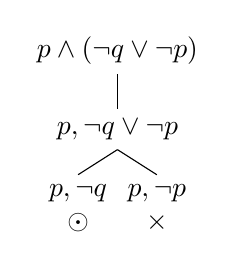
\begin{tikzpicture}[
        level distance=1cm,
        sibling distance=1.5cm,
        level 2/.style={sibling distance=1cm},
        edge from parent path={(\tikzparentnode.south) -- (\tikzchildnode.north)}
      ]
      \node {$p \land (\neg q \lor \neg p)$}
        child { 
          node {$p, \neg q \lor \neg p$}
          child { node[align=center] {$p, \neg q$ \\ $\odot$} }
          child { node[align=center] {$p, \neg p$ \\ $\times$} }
        };
      \end{tikzpicture}
      }  
    \end{latin}
  \end{center}
  شاخهٔ \(p,\neg q\) باز است با \(p=T,\,q=F\) که مدلی برای \(A\) می‌سازد.
  \end{example}
  
  \begin{example}[مثال \lr{2.74}]
  فرض کنید
  \[
    A = p \lor (q\land\neg q).
  \]
  یک جدول ممکن:
  \begin{center}
    \begin{latin}
      \resizebox{0.35\textwidth}{!}{
      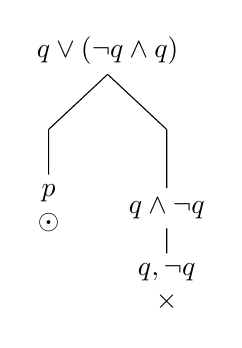
\begin{tikzpicture}[
        level distance=1cm,
        sibling distance=1.5cm,
        level 2/.style={sibling distance=1cm},
        edge from parent path={(\tikzparentnode.south) -- (\tikzchildnode.north)}
      ]
      \node {$q \lor (\neg q \land q)$}
        child { 
          child { node[align=center] {$p$ \\ $\odot$} }
        }
        child { 
          child { 
            node {$q \land \neg q$}
            child { node[align=center] {$q, \neg q$ \\ $\times$} }
          }
        };
      \end{tikzpicture}
      }  
    \end{latin}
  \end{center}
  شاخهٔ \(p\) باز است، پس هر مدلی باید \(p=T\) باشد.
  \end{example}
  
  \begin{theorem}[قضیهٔ \lr{2.77}]
  اگر \(l\) یک برگ باز در جدول تکمیل‌شده \(T\) باشد، آنگاه
  \[
    U \;=\;\bigcup_{i\in\text{شاخه از ریشه تا }l} U(i)
  \]
  یک مجموعهٔ هینتیکا است.
  \end{theorem}
  \begin{proof}
  \begin{enumerate}[1)]
    \item لیترال‌ها در هیچ قاعده‌ای شکسته نمی‌شوند و از ریشه تا برگ منتقل می‌گردند. چون برگ باز است، جفت متضاد در \(U(l)\) نیست، پس شرط (1) برقرار است.
    \item اگر \(A\in U\) یک \(\alpha\)-فرمول باشد، در مسیر تجزیه شده و زیرفرمول‌های \(A_1,A_2\) در \(U\) قرار می‌گیرند.
    \item اگر \(B\in U\) یک \(\beta\)-فرمول باشد، در مسیر تجزیه شده و یکی از زیرفرمول‌های \(B_1\) یا \(B_2\) در \(U\) قرار می‌گیرد.
  \end{enumerate}
  بنابراین \(U\) هینتیکا است.
  \end{proof}
  
  \begin{theorem}[لم هینتیکا \lr{2.78}]
  اگر \(U\) یک مجموعهٔ هینتیکا باشد، آنگاه \(U\) برآورده‌پذیر است.
  \end{theorem}
  \begin{proof}
  اتم‌های \(P_U\) را مجموعهٔ اتم‌های ظاهرشده در \(U\) در نظر بگیرید. تفسیر
  \(\mathscr{I}\) را تعریف می‌کنیم:
  \[
  \mathscr{I}(p)=
  \begin{cases}
  \mathsf{T}, & p\in U,\\
  \mathsf{F}, & \neg p\in U,\\
  \mathsf{T}, & \text{اگر }p,\neg p\notin U.
  \end{cases}
  \]
  شرط (1) تناقض را نفی می‌کند. سپس با استقرا بر ساختار فرمول‌ها نشان می‌دهیم برای هر \(A\in U\)، \(v_{\mathscr{I}}(A)=\mathsf{T}\):
  \begin{itemize}
    \item اگر \(A=p\) یا \(A=\neg p\)، واضح است.
    \item اگر \(A=A_1\land A_2\)، شرط (2) هر دو \(A_1,A_2\in U\) را تضمین می‌کند.
    \item اگر \(A=B_1\lor B_2\)، شرط (3) یکی از آنها را تضمین می‌کند.
  \end{itemize}
  پس \(\mathscr{I}\) مدلی از \(U\) است.
  \end{proof}
  
  \subsubsection*{نتیجه‌گیری}
  اگر \(T\) جدولی باز و تکمیل‌شده برای \(A\) باشد، اجتماع برچسب‌های شاخهٔ باز مجموعه‌ای هینتیکا می‌سازد (قضیهٔ \lr{2.77}) و از لم هینتیکا (قضیهٔ \lr{2.78}) این مجموعه مدل دارد. چون \(A\) در برچسب ریشه هست، \(\mathscr{I}\) مدلی برای \(A\) می‌شود و بنابراین اثبات کامل بودن پایان می‌یابد.